\documentclass[a4paper,12pt]{article}

\usepackage[utf8]{inputenc}
\usepackage[T1]{fontenc}
\usepackage[a4paper,total={150mm,240mm}]{geometry}
\usepackage{amsmath}
\usepackage{amsfonts}
\usepackage{amsthm}
\usepackage{amscd}
\usepackage{grffile}
\usepackage{tikz}
\usepackage{eurosym}
\usepackage{graphicx}
\usepackage{color}
\usepackage{listings}
\lstset{language=C++, basicstyle=\ttfamily,
  keywordstyle=\color{black}\bfseries, tabsize=4, stringstyle=\ttfamily,
  commentstyle=\itshape, extendedchars=true, escapeinside={/*@}{@*/},
  rangebeginprefix = ///\ tex:\ ,
  rangeendprefix   = ///\ tex:\ ,
  includerangemarker=false }
\usepackage{paralist}
\usepackage{curves}
\usepackage{calc}
\usepackage{picinpar}
\usepackage{enumerate}
\usepackage{algpseudocode}
\usepackage{bm}
\usepackage{multibib}
\usepackage{hyperref}
\usepackage{textcase}
\usepackage{nicefrac}
\usepackage{stmaryrd}
\usepackage{showkeys}

\theoremstyle{definition}
\newtheorem{Def}{Definition}
\newtheorem{Thm}[Def]{Theorem}
\newtheorem{Prop}[Def]{Proposition}
\newtheorem{Lem}[Def]{Lemma}
\theoremstyle{definition}
\newtheorem{Exm}[Def]{Example}
\newtheorem{Obs}[Def]{Observation}
\newtheorem{Pro}[Def]{Proposition}
\newtheorem{Cor}[Def]{Corollary}
\newtheorem{Rem}[Def]{Remark}
\newtheorem{Alg}[Def]{Algorithm}

\DeclareMathOperator{\argmin}{argmin}
\DeclareMathOperator{\diam}{diam}
\DeclareMathOperator{\convexhull}{convex\,hull}
\DeclareMathOperator{\mathspan}{span}
\DeclareMathOperator{\tridiag}{tridiag}
\DeclareMathOperator{\diag}{diag}
\DeclareMathOperator{\FE}{FE}
\DeclareMathOperator{\supp}{supp}
\DeclareMathOperator{\esssup}{ess\,sup}

\newcommand{\N}{\mathbb{N}}
\newcommand{\Z}{\mathbb{Z}}
\newcommand{\R}{\mathbb{R}}
\newcommand{\C}{\mathbb{C}}
\newcommand{\Q}{\mathbb{Q}}
\newcommand{\B}{\mathbb{B}}
\newcommand{\K}{\mathbb{K}}
\newcommand{\intt}{\int\limits}
\newcommand{\delt}{\Delta t}
\newcommand{\Dim}{d}

\def\dx{\mathrm{d}\,x}

\definecolor{listingbg}{gray}{0.95}

\title{DUNE PDELab Tutorial 07 \\
Discontinuous Galerkin Method for Hyperbolic conservation laws}
\author{DUNE/PDELab Team}
\date{\today}

\begin{document}

\maketitle
\tableofcontents
\clearpage

\section{Introduction}

In this tutorial we provide  DG solver for hyperbolic conservation laws. As an example of hyperbolic system we consider: linear acoustics, shallow water equation, 
treatment of systems of hyperbolic partial differential equations in PDELab.

\section{PDE Problem}

We are interested in the numerical solution to the first-order
hyperbolic partial differential equations (PDEs). The general conservative form of the hyperbolic problem,  for  the unknown $u\in\mathbb{R}^m$
reds as follows
\begin{equation}
\label{eq:master_problem}
\partial_t u(x,t) + \nabla\cdot F(u(x,t),x,t) = g(u(x,t),x,t)  \quad\text{in $U=\Omega\times\Sigma$} ,
\end{equation}
where the matrix-valued function $F : \mathbb{R}^m\times\Omega\times\Sigma \to \mathbb{R}^{m\times \Dim}$
with the columns $F(u,x,t) = [F_1(u,x,t),\ldots,F_d(u,x,t)]$ is called \textit{flux function}.
Note that the divergence is defined as $\nabla\cdot F(u(x,t),x,t) = \sum_{j=1}^{\Dim} \partial_{x_j} F_j(u(x,t),x,t)$.
Moreover let $\Omega=\mathbb{R}^{\Dim}$, $\Dim\in\mathbb{N}$ is the spatial domain,  and $\Sigma=\mathbb{R}^+$ is the temporal domain. Equation \eqref{eq:master_problem} is supplemented with initial conditions
\begin{equation*}
u(x,0) = u_0(x) .
\end{equation*}

%hyperbolicity - copy from Bangkok School Lecture Notes
Equation \eqref{eq:master_problem} is said to be in \textit{conservative form} as it arises naturally
from the formulation of conservation of mass, momentum and energy.
If the flux function is smooth enough, the PDE can be put in its \textit{non-conservative}
or \textit{quasi-linear} form which reads
\begin{equation}
\label{eq:master_nonconservative_form}
\partial_t u(x,t) + \sum_{j=1}^{\Dim} B_j(u(x,t),x,t) \partial_{x_j} u(x,t) + \tilde{g}(u(x,t),x,t) = 0
\quad\text{in $\Omega\times\Sigma$} .
\end{equation}
The reason is the chain rule
\begin{align*}
\partial_{x_j} F_{i,j}(u(x,t),x,t) = \sum_{k=1}^m \frac{\partial F_{i,j}}{\partial u_k}( u(x,t),x,t)
\frac{\partial u_k}{\partial x_j} (x,t) + \frac{\partial F_{i,j}}{\partial x_j} (u(x,t),x,t)
\end{align*}
which shows
\begin{align*}
\left(B_j(u,x,t)\right)_{i,k} &= \frac{\partial F_{i,j}}{\partial u_k}(u,x,t), &
\tilde{g}_i(u,x,t) &= g_i(u,x,t) + \frac{\partial F_{i,j}}{\partial x_j} (u ,x,t) .
\end{align*}


It turns out that many systems of the form \eqref{eq:master_nonconservative_form}
which are of practical interest satisfy an important property that is essential in the theoretical and numerical treatment.
\begin{Def}[Hyperbolic First-Order PDE]\label{def:HyperbolicSystems}
	The system of equations \eqref{eq:master_nonconservative_form} is called \textit{hyperbolic} if
	for each feasible state $u\in\mathbb{R}^m$, $x\in\Omega$, $t\in\Sigma$ and
	$y\in\mathbb{R}^{\Dim}$ the $m\times m$ matrix
	\begin{equation}\label{eq:BMatrix}
	B(u,x,t; y) = \sum_{j=1}^{\Dim} y_j B_j(u,x,t)
	\end{equation}
	is real diagonalizable, i.e. $B(u,x,t;y)$ has $m$ real eigenvalues $\lambda_1(x,t;y), \ldots, \lambda_m(x,t;y)$
	and its corresponding right eigenvectors $r_1(x,t;y), \ldots, r_m(x,t;y)$ form a basis of $\mathbb{R}^m$.
	In addition there are the special cases:
	\begin{enumerate}[i)]
		\item The system is called \textit{symmetric hyperbolic} if $B_j(u,x,t)$ is symmetric for every
		feasible state $u\in\mathbb{R}^m$, $x\in\Omega$, $t\in\Sigma$ and $j=1,\ldots,m$.
		\item The system is called \textit{strictly hyperbolic} if all $m$ eigenvalues are distinct for
		every feasible state $u\in\mathbb{R}^m$, $x\in\Omega$, $t\in\Sigma$. $\hfill\square$
	\end{enumerate}
\end{Def}
Note that the definition of hyperbolicity relies on the non-conservative form.


For the sake of brevity we omit theoretical discussion.
Interested reader can find vast literature on hyperbolic PDEs, good start would be \cite[Chapter 11]{Evans}.
%\cite{Peter _script}

In the subsequent Sections we will give three examples of hyperbolic systems: linear acoustics, shallow water equations, and Maxwell's equations. We formulate corresponding PDEs in conservative form \eqref{eq:master_problem} and provide properties necessary to develop numerical schemes.

\subsection{Acoustic Wave Equation}\label{sec:SoundWaves}



The acoustic wave equation governs the propagation of acoustic waves through a material medium. Linearizing mass and momentum equations around the background state, dropping all higher-order terms in fluctuations and assuming \textit{constant background pressure} results (without external sources) in
\begin{subequations}\label{eq:LinearAcoustics1}
	\begin{align}
	\partial_t \tilde{\rho} +  \nabla\cdot(\bar{\rho} \tilde{v}) &= 0, &&\text{(conservation of mass)}\\
	\partial_t (\bar\rho \tilde{v}) + \nabla \tilde{p} &= 0, &&\text{(conservation of momentum)}.
	\end{align}
\end{subequations}

It should be noted that it is the first order system that is derived from the physics and not
the scalar second order wave equation, see also \cite[§ 2.7]{LeVeque}.

\paragraph{Conservative Form of Linear Acoustics}

We now consider the case that the speed of sound $c$ is \textit{piecewise constant} in
fixed subdomains (e.g. due to temperature variations).
Equation \eqref{eq:LinearAcoustics1} is still valid in this case since only
$\bar{p}$ being constant has been assumed.
We conclude that pressure $\tilde{p}$ and normal momentum
$\bar{\rho} \tilde{v}\cdot n$ are continuous
at subdomain boundaries where $c$ is discontinuous (this follows from integration by parts
at enforcing continuity of mass and momentum at the subdomain boundaries).

Due to $\rho = p/c^2 = (\bar{p} + \tilde{p})/c^2 = \bar{p}/c^2 +\tilde{p}/c^2 = \bar\rho + \tilde\rho$
also the background density $\bar\rho$ is piecewise constant. In case of varying speed of sound
it is then more appropriate to use the conservative variables $(\tilde\rho, \bar{\rho} \tilde{v}) = (\tilde\rho,\tilde{q})$
resulting in the system
\begin{subequations}\label{eq:LinearAcousticsConservative}
	\begin{align}
	\partial_t \tilde{\rho} +  \nabla\cdot\tilde{q} &= 0,\\
	\partial_t \tilde{q} + \nabla (c^2\tilde{\rho}) &= 0.
	\end{align}
\end{subequations}
At subdomain boundaries where $c$ is discontinuous $c^2\tilde\rho$
(which is the pressure) and $\tilde{q}\cdot n$ are continuous.

Let us rewrite \eqref{eq:LinearAcousticsConservative} at conservative hyperbolic system. Note that number of components $m=\Dim+1$
$$\partial_t u(x,t) + \nabla\cdot F(u(x,t),x,t) = 0,$$
where 
$$u = (\varrho,q_1,\dots,\Dim) $$
and 
$$F(u(x,t),x,t) = \left( \begin{smallmatrix}
q_1  & q_2 & \dots & q_\Dim\\
c^2\rho & 0 & \dots & 0\\
0 & c^2\rho & \dots & 0\\
\vdots & \vdots & \ddots & \vdots\\
0 & 0 & \dots & c^2\rho 
\end{smallmatrix} \right)\in \mathbb{R}^{m\times \Dim} $$

Linear Acoustics problem has the two nonzero eigenvalues $\pm c$.


\subsection{Shallow Water Equations}
The Shallow Water model is the system of nonlinear hyperbolic PDEs, more precisely conservation law that describes the evolution of the height and the mean velocity of the fluid. It is widely used for predictions of flooding, dam-breaks, tsunamis or free oscillations of water. Another application of the Shallow Water Equations is long term simulations of the flow in rivers.

In 2d SWE reads as follows (number of components $m=\Dim+1=3$)
\begin{equation}\label{eq:swe2D}
\partial_t \begin{pmatrix}
h\\
u_1h\\
u_2h
\end{pmatrix}+ \nabla\cdot
\left( \begin{matrix}
u_1h   & u_2h\\
u_1^2h + \frac{1}{2}gh^2 & u_1u_2h\\
u_1u_2h & u_2^2h + \frac{1}{2}gh^2
\end{matrix}\right) = 0,
\end{equation}
Where $h>0$ stands for water height, and $u=(u_1,u_2)$ is the velocity.

In conservative variables $q = (h, u_1h,u_2h)$ system \eqref{eq:swe2D} reads
To show the hyperbolicity, we need the non-conservative form of \eqref{eq:swe2D:repeat}.
Therefore we rewrite the equation and introduce conservative variables as in the previous Chapter to obtain
\begin{align} 
&\partial_t\begin{pmatrix}
q_1\\
q_2\\
q_3
\end{pmatrix} + 
\nabla \cdot \left( \begin{matrix}
q_2 & q_3\\
q_2^2/q_1 + \frac{1}{2}gq_1^2 & \frac{q_2q_3}{q_1}\\
\frac{q_2q_3}{q_1} & q_3^2/q_1 + \frac{1}{2}gq_1^2
\end{matrix} \right) = 0.
\end{align}
This modes have three distinct eigenvalues for $h\neq 0$ and therefore the two dimensional Shallow Water Equations are a strictly hyperbolic system for wet domains (i.e. $h>0 \forall (x,t) \in \Omega\times\Sigma$).

In this tutorial we also consider 1d SWE. This is not physical explanation by one can see the 1d SWE as 2x2 block of 2d flux matrix.

\subsection{Maxwell's Equations}


Maxwell's equations are a set of PDS that underpin all electric, optical and radio technologies, including power generation, electric motors, wireless communication, cameras, televisions, computers etc. Maxwell's equations describe how electric and magnetic fields are generated by charges, currents, and changes of each other. 

The Maxwell system is given by
\begin{subequations}
	\begin{align}
	\partial_t D - \nabla\times H &= -J, &&\text{(Ampère)} \label{eq:Ampere}\\
	\partial_t B + \nabla\times E &= 0, &&\text{(Faraday)} \label{eq:Faraday}\\
	\nabla\cdot D &= \rho, &&\text{(Gauß)} \label{eq:Gauss1}\\
	\nabla\cdot B &=0, &&\text{(Gauß for magnetism)} \label{eq:Gauss2}
	\end{align}
\end{subequations}
together with the constitutive laws
\begin{subequations}
	\begin{align}
	D &= \epsilon E, &&\text{( $\epsilon$. permittivity)}\\
	B &= \mu H, &&\text{( $\mu$: permeability)}\\
	J &= \sigma E + j, &&\text{( $\sigma$: conductivity)} .
	\end{align}
\end{subequations}
The following vector fields in $\mathbb{R}^3$ need to be determined:
\begin{center}
	\begin{tabular}{lll}
		Symbol & Name & Unit\\
		\hline
		$B$ & magnetic flux density & $\frac{Vs}{m^2}$\\
		$H$ & magnetic field intensity & $\frac{A}{m}$\\
		$E$ & electric field intensity & $\frac{V}{m}$\\
		$D$ & displacement current density & $\frac{AS}{m^2}$\\
		\hline
	\end{tabular}
\end{center}
whereas the scalar charge density $\rho$ and the current density $j$ are prescribed.

The conditions \eqref{eq:Gauss1} and \eqref{eq:Gauss1} are needed only for the
initial condition. The evolution in time is described by \eqref{eq:Faraday} and
\eqref{eq:Ampere} only, see \cite{JinBook}.

Since $D$ and $B$ are conserved quantities we formulate equations \eqref{eq:Faraday} and
\eqref{eq:Ampere} in terms of $D$ and $B$ using the constitutive equations:
\begin{subequations}
	\begin{align}
	\partial_t D - \nabla\times\left(\frac{1}{\mu} B\right) + \frac{\sigma}{\epsilon} D &= - j\,,  \\
	\partial_t B + \nabla\times\left( \frac{1}{\epsilon} D \right) &= 0\, .
	\end{align}
\end{subequations}
Writing out the curl operator $\nabla\times$ and defining the six component
vector $u=(D_1,D_2,D_3,B_1,B_2,B_3)^T$ we obtain the linear hyperbolic system
\begin{equation}
\partial_t u + \sum_{j=1}^3 B_j \partial_{x_j} u + C u = q
\end{equation}
with
\begin{align*}
B_1 &= \left( \begin{array}{ccc|ccc}
0 & 0 & 0 & 0 & 0 & 0\\ 
0 & 0 & 0 & 0 & 0 & \nicefrac{1}{\mu}\\ 
0 & 0 & 0 & 0 & \nicefrac{-1}{\mu} & 0\\ 
\hline
0 & 0 & 0 & 0 & 0 & 0\\ 
0 & 0 & \nicefrac{-1}{\epsilon} & 0 & 0 & 0\\ 
0 & \nicefrac{1}{\epsilon} & 0 & 0 & 0 & 0
\end{array}
\right), &
B_2 &= \left( \begin{array}{ccc|ccc}
0 & 0 & 0 & 0 & 0 & \nicefrac{-1}{\mu}\\ 
0 & 0 & 0 & 0 & 0 & 0\\ 
0 & 0 & 0 & \nicefrac{1}{\mu} & 0 & 0\\ 
\hline
0 & 0 & \nicefrac{1}{\epsilon} & 0 & 0 & 0\\ 
0 & 0 & 0 & 0 & 0 & 0\\ 
\nicefrac{-1}{\epsilon} & 0 & 0 & 0 & 0 & 0
\end{array}
\right),\\
B_3 &= \left( \begin{array}{ccc|ccc}
0 & 0 & 0 & 0 & \nicefrac{1}{\mu} & 0\\ 
0 & 0 & 0 & \nicefrac{-1}{\mu} & 0 & 0\\ 
0 & 0 & 0 & 0 & 0 & 0\\ 
\hline
0 & \nicefrac{-1}{\epsilon} & 0 & 0 & 0 & 0\\ 
\nicefrac{1}{\epsilon} & 0 & 0 & 0 & 0 & 0\\ 
0 & 0 & 0 & 0 & 0 & 0
\end{array}
\right), &
C &= \left( \begin{array}{ccc|ccc}
\nicefrac{\sigma}{\epsilon} & 0 & 0 & 0 & 0 & 0\\ 
0 & \nicefrac{\sigma}{\epsilon} & 0 & 0 & 0 & 0\\ 
0 & 0 & \nicefrac{\sigma}{\epsilon} & 0 & 0 & 0\\ 
\hline
0 & 0 & 0 & 0 & 0 & 0\\ 
0 & 0 & 0 & 0 & 0 & 0\\ 
0 & 0 & 0 & 0 & 0 & 0
\end{array}
\right),
\end{align*}
and $q=(-j_1,-j_2,-j_3,0,0,0)^T$. Hyperbolicity is obtained from the 
matrix
\begin{equation}
B_\text{Maxwell}(y) = \sum_{j=1}^{3} y_jB_j = \left( \begin{array}{ccc|ccc}
0 & 0 & 0 & 0 & \nicefrac{y_3}{\mu} & \nicefrac{-y_2}{\mu}\\ 
0 & 0 & 0 & \nicefrac{-y_3}{\mu} & 0 & \nicefrac{y_1}{\mu}\\ 
0 & 0 & 0 & \nicefrac{y_2}{\mu} & \nicefrac{-y_1}{\mu} & 0\\ 
\hline
0 & \nicefrac{-y_3}{\epsilon} & \nicefrac{y_2}{\epsilon} & 0 & 0 & 0\\ 
\nicefrac{y_3}{\epsilon} & 0 & \nicefrac{-y_1}{\epsilon} & 0 & 0 & 0\\ 
\nicefrac{-y_2}{\epsilon} & \nicefrac{y_1}{\epsilon} & 0 & 0 & 0 & 0
\end{array}
\right) .
\end{equation}
Using the diagonal transformation matrix 
$$T=\text{diag}(\sqrt{\nicefrac{1}{\epsilon}},\sqrt{\nicefrac{1}{\epsilon}},\sqrt{\nicefrac{1}{\epsilon}},
\sqrt{\nicefrac{1}{\mu}},\sqrt{\nicefrac{1}{\mu}},\sqrt{\nicefrac{1}{\mu}})$$
we obtain the similarity transformation
\begin{equation}
T B_\text{Maxwell}(y) T^{-1} =
\frac{1}{\sqrt{\epsilon\mu}}\left( \begin{array}{ccc|ccc}
0 & 0 & 0 & 0 & y_3 & -y_2\\ 
0 & 0 & 0 & -y_3 & 0 & y_1\\ 
0 & 0 & 0 & y_2 & -y_1 & 0\\ 
\hline
0 & -y_3 & y_2 & 0 & 0 & 0\\ 
y_3 & 0 & -y_1 & 0 & 0 & 0\\ 
-y_2 & y_1 & 0 & 0 & 0 & 0
\end{array}
\right) .
\end{equation}
Thus $B_\text{Maxwell}(y)$ is similar to a real symmetric matrix from which the
set of eigenvalues and eigenvectors can be determined.
It turns out that the eigenvalues 
of $B_\text{Maxwell}(y)$ are $0$, $c\|y\|$ and $c\|y\|$ each with
multiplicity $2$ and $c=\nicefrac{1}{\sqrt{\epsilon\mu}}$ the speed of light.


\section{Discontinuous Galerkin Methods}

In this section we present a numerical method to solve the original
problem \eqref{eq:master_problem} which is repeated for convenience here.
Let $u: \Omega\times\Sigma\to\mathbb{R}^m$ be the solution of the
hyperbolic first-order system
\begin{subequations}
	\label{eq:master_problem_repeated}
	\begin{align}
	\partial_t u(x,t) + \nabla\cdot F(u(x,t),x,t) &= f(u(x,t),x,t), &&\text{in $U=\Omega\times\Sigma$}, \\
	u(x,t) &= u_0(x), &&\text{at $t=0$},
	\end{align}
\end{subequations}
where $\Omega\subset\mathbb{R}^{\Dim}$ is a bounded domain, $\Sigma=(t_0,t_0+T)$
is a time interval of interest and $F(u,x,t)=[F_1(u,x,t),\ldots,F_n(u,x,t)]$ is the
matrix valued flux function with columns $F_j(u,x,t)$.

\subsection{Space Discretization with Discontinuous Galerkin}

For any test function $v$ being piecewise smooth
on the mesh $\mathcal{E}_h$ there holds
\begin{equation}\label{eq:DG_identity}
\begin{split}
\int_\Omega \biggl[&\partial_t u + \sum_{j=1}^{\Dim}\partial_{x_j}F_j(u,x,t)\biggr]\cdot v \,dx = \\
&= d_t (u,v)_\Omega + \sum_{e\in\mathcal{E}_h} \sum_{j=1}^{\Dim} \sum_{i=1}^m
\int_e (\partial_{x_j}F_{i,j}(u,x,t)) \, v_i \,dx \\
&= d_t (u,v)_\Omega + \sum_{e\in\mathcal{E}_h} \sum_{j=1}^{\Dim} \sum_{i=1}^m
\biggl[ - \int_e F_{i,j}(u,x,t) \,\partial_{x_j} v_i \,dx \\
&\qquad+ \int_{\partial e} F_{i,j}(u,s,t) v_i n_j\,ds \biggr]\\
&= d_t (u,v)_\Omega + \sum_{e\in\mathcal{E}_h}  \biggl[-\int_e F(u,x,t) : \nabla v\,dx
+ \int_{\partial e} (F(u,s,t)n)\cdot v\,ds\biggr]\\
&= d_t (u,v)_\Omega - \sum_{e\in\mathcal{E}_h} \int_e F(u,x,t) : \nabla v\,dx\\
&\qquad + \sum_{f\in\mathcal{F}_h^i} \int_f \llbracket (F(u,s,t)n)\cdot v \rrbracket \,ds
+ \sum_{f\in\mathcal{F}_h^{\partial\Omega}} \int_f (F(u,s,t)n)\cdot v \,ds \,.
\end{split}
\end{equation}

\section{Numerical Fluxes}


Next step is to construct a numerical flux function. Since the space of discrete solutions $u_h\in V_h$, is not single-valued on the interface the normal flux $ F(\mathbf{u}, \mathbf{x}, t)\cdot~\mathbf{n} $ is not well-defined.
Hence for all $S \in \mathcal{F}$, $\mathbf{u}$ is split up to the so called left and right states, 
\begin{equation}\label{eq:statesplitting}
\begin{matrix}
\mathbf{u}_S^- := \left\lbrace
\begin{array}{ll}
\mathbf{u}\vert_{T_1} & \mathrm{if}\ S \in \mathcal{F}^i, \\
\mathbf{u}\vert_T & \mathrm{if}\ S \in \mathcal{F}^{\partial \Omega},
\end{array} \right.
& \mathbf{u}_S^+ := \left\lbrace
\begin{array}{ll}
\mathbf{u}\vert_{T_2} & \mathrm{if}\ S \in \mathcal{F}^i, \\
b & \mathrm{if}\ S \in \mathcal{F}^{\partial \Omega},
\end{array}\right.
\end{matrix}
\end{equation}

where $T_1$ and $T_2$ are the two elements sharing the interface $S \in \mathcal{F}^i$,\\ i.e. \mbox{$\partial T1 \cup \partial T2 = S$},  and \mbox{$b=b(s,t):\partial\Omega\times\Sigma\rightarrow \mathbb{R}^m $} is an external state enforced by a boundary condition.
How to define the numerical flux depends on the linearity of equation \eqref{eq:sysDG}. Besides, effects like numerical diffusion and the desired stability must be considered.
In general, a numerical flux is defined as a function
\begin{align}
\Phi :  \mathbb{R}^d \times U \times U \rightarrow \mathbb{R},
\end{align}
which provides a single-valued approximation of $F \cdot \mathbf{n}_S$ if we set the first argument to $\mathbf{n}_S$, for detailed description we refer to \cite{DiPietro}.

In order to obtain physically correct approximations of the solution a numerical flux has to comply with the following properties:

\subsubsection{Consistency of numerical fluxes}
\begin{Def}\label{def:flux:consistency}
	A numerical flux $\Phi$ is called consistent, if it is linear in its first argument, Lipschitz continuous with respect to the second and third argument and if for all $n\in \mathbb{R}^d, v\in U$ it holds
	\begin{align}
	\Phi(n,v,v) = F(v)\cdot \mathbf{n}.
	\end{align}
\end{Def}

That means it is exact if the solution is continuous between two neighboring elements.

\subsubsection{Conservation of numerical fluxes}
A numerical flux $\Phi$ needs to be conservative, i.e. 
\begin{equation}
\Phi(n_1,u_1,u_2) + \Phi(n_2, u_2, u_1) = 0,
\end{equation}
where $u_1$ and $u_2$ are the states on elements $T_1, T_2$ sharing an edge $S$ and $n_1$ (resp. $n_2$) is the unit outer normal of $T_1$ (resp. $T_2$) on $S$, thus it holds $n_1 = -n_2$. 

\subsection{Local Lax-Friedrichs}

For nonlinear problems a possible choice is the local Lax-Friedrichs flux, 
\begin{equation}
\Phi (n_S, \mathbf{u}^-, \mathbf{u}^+) = \frac{1}{2}(F(\mathbf{u}^-)\cdot n_S + F(\mathbf{u}^+)\cdot n_S - \alpha (\mathbf{u}^+ -\mathbf{u}^- )),
\end{equation}
where $\alpha$ is an estimate of the largest absolute value of the eigenvalues of the Jacobian $\partial_u F(u)\cdot n$ in a neighbourhood of the edge S.
For hyperbolic systems, we can calculate these eigenvalues as we did in Chapter \ref{ch:modelSWE}.
For the 1D SWE we have the eigenvalues $\lambda_{1,2} = u \pm \sqrt{gh}$, depending on the physical variables $u$ and $h$.
Thus $\vert u \vert +\sqrt{gh}$ is the largest absolute value for one state and as we are interested in the maximum in a neighbourhood of $S$, we choose $\alpha = \max\limits_{\mathbf{u}^-, \mathbf{u}^+} \vert u \vert +\sqrt{gh}$.
For the two dimensional case, we get similarly $\alpha = \max\limits_{\mathbf{u}^-, \mathbf{u}^+} \vert n^Tu \vert +\sqrt{gh}$, where $n$ is the unit outer normal vector of one of the elements.


\subsection{Flux Vector Splitting}

Here we only consider the linear 
constant coefficient case $F_j(u) = B_j u$. Then the normal flux is
\begin{equation}
F(u,x,t)n = \sum_{j=1}^{\Dim} F_j(u) n_j = \sum_{j=1}^{\Dim} (B_j u) n_j
=\left( \sum_{j=1}^{\Dim} n_j B_j\right) u = B_n u \, .
\end{equation}
Due to hyperbolicity the matrix $B_n = \left( \sum_{j=1}^{\Dim} n_j B_j\right)$
is real diagonalizable for all $n\in\mathbb{R}^{\Dim}$ and we may use the numerical flux function
\eqref{eq:system_upwind} based on flux vector splitting:
\begin{equation}
\Phi_U(u,B_n)(x) = B_n^+ u^-(x) + B_n^- u^+(x) .
\end{equation}

In order to achive higher order we employ a finite element space with higher-order polynomials:
\begin{equation}
V_h^q = \left\{ v\in L^2(\Omega) \,:\, 
v|_e = p\circ\mu_e^{-1}, p\in\mathbb{P}^{q,d}\right\}
\end{equation}
where the differentiable and invertible map $$\mu_e : \hat{E} \to e$$
maps the reference element $\hat{E}$ to an element $e\in\mathcal{E}_h$ and the multivariate
polynomials of degree $q$ in $d$ space dimensions are given by
\begin{equation*}
\mathbb{P}^{q,d} = \left\{\begin{array}{ll}
\left\{ p\,:\, p(x_1,\ldots,x_d) = \sum\limits_{0\leq\|\alpha\|_1\leq q} c_\alpha
x_1^{\alpha_1}\cdot\ldots\cdot x_d^{\alpha_d}\right\} & \text{($\hat{E}$ simplex)}, \\
\left\{ p\,:\, p(x_1,\ldots,x_d) = \sum\limits_{0\leq\|\alpha\|_\infty\leq q} c_\alpha
x_1^{\alpha_1}\cdot\ldots\cdot x_d^{\alpha_d}\right\} & \text{($\hat{E}$ cube)},
\end{array}\right .
\end{equation*}
depending on the type of element.

The upwind semi-discrete scheme for multi-dimensional linear hyperbolic systems then reads
as follows. Find $u_h : \Sigma\to (V_h^q)^m$ s. t.:
\begin{equation}\label{eq:DG_identity}
\begin{split}
d_t (u&,v)_\Omega + b_{DG}(u(t),v) = l_{DG}(v) \,,
\end{split}
\end{equation}
where the DG spatial bilinear form is given by
\begin{equation}\label{eq:DG_blf}
\begin{split}
b_{DG}(u,v) &= -\sum_{e\in\mathcal{E}_h} \int_e F(u,x,t) : \nabla v\,dx\\
&\quad +\sum_{f\in\mathcal{F}_h^i} \int_f (B_n^+ u^-(s,t) + B_n^- u^+(s,t)) 
\cdot \llbracket  v \rrbracket \,ds\\
&\quad + \sum_{f\in\mathcal{F}_h^{\partial\Omega}} \int_f 
(B_n^+ u^-(s,t)) \cdot v \,ds
\end{split}
\end{equation}
and the right hand side by
\begin{equation}\label{eq:DG_rhs}
\begin{split}
l_{DG} =  (f(t),v)_\Omega - \sum_{f\in\mathcal{F}_h^{\partial\Omega}} \int_f 
(B_n^- g(s,t))\cdot v \,ds \, .
\end{split}
\end{equation}

\paragraph{Boundary flux}

The boundary flux can be used to implement various boundary conditions:

\begin{itemize}
	\item Absorbing boundary conditions
	$$B_n^+ u^-(s,t)$$
	\item Incoming wave
	$$B_n^+ u^-(s,t) + B_n^- g(s,t) $$
	\item Reflecting boundary conditions\\
	$$B_n^+ u^-(s,t) + B_n^- u^-(s,t) $$
\end{itemize}

\section{Riemann Solvers}

\subsection*{Constant Coefficient Case}

The upwind flux \eqref{eq:system_upwind} can be interpreted with the help of the solution of the
following so-called \textit{Riemann problem}:
\begin{align*}
\partial_t u(x,t) + \partial_x (B u(x,t)) &= 0, &&(\text{in $\mathbb{R}\times\mathbb{R}^+$})\\
u(x,0) &= \left\{\begin{array}{ll}
U_L & x \leq 0\\ U_R & x > 0
\end{array}\right ., &&(t=0)\,.
\end{align*}
Riemann problems are characterized by an initial condition with two
constant states and a discontinuity at $x=0$. Here we assume that $B$ is a constant matrix.

The solution of this Riemann problem can be constructed according to
the discussion in Section \ref{sec:one_d_system}.
First, transform the left and right states to characteristic variables:
$W_L = R^{-1}U_L$ and $W_R = R^{-1}U_R$. Let the eigenvalues be sorted
with $k$ eigenvalues negative and $m-k$ eigenvalues non-negative (there may
be zero eigenvalues):
$$ \lambda_1 \leq \lambda_2 \leq \ldots \leq\lambda_k < 0
\leq \lambda_{k+1} \leq \ldots \leq \lambda_m \,.  $$
Then the solution is piecewise constant in space time cones as follows:
\begin{center}
	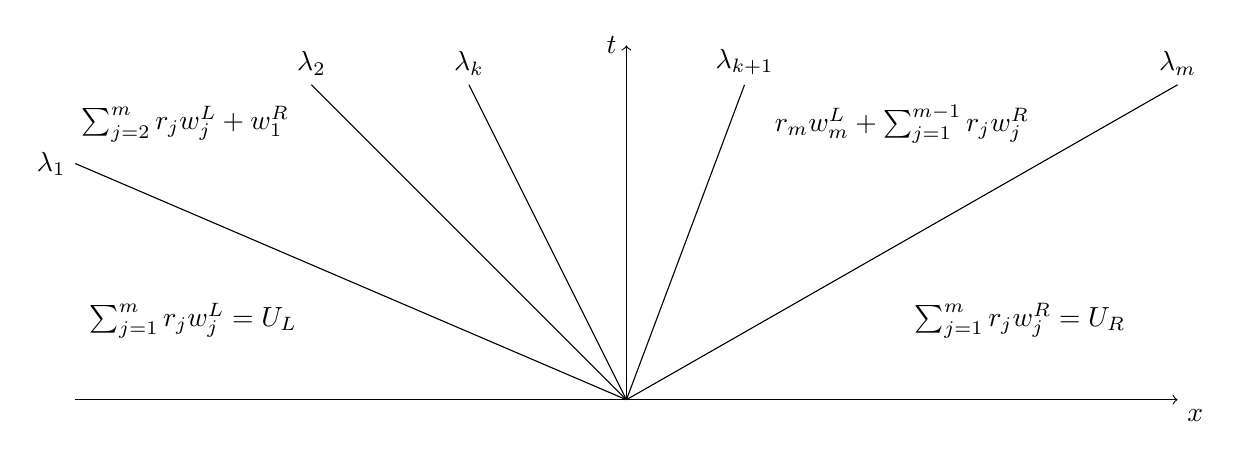
\begin{tikzpicture}[scale=1.0]
	\draw[->] (-7,0) -- (7,0) node[below right] (n) {$x$};
	\draw[->] (0,0) -- (0,4.5) node[left] (n) {$t$};
	\draw (0,0) -- (-7,3) node[left] (n) {$\lambda_1$};
	\draw (0,0) -- (-4,4) node[above] (n) {$\lambda_2$};
	\draw (0,0) -- (-2,4) node[above] (n) {$\lambda_k$};
	\draw (0,0) -- (1.5,4) node[above] (n) {$\lambda_{k+1}$};
	\draw (0,0) -- (7,4) node[above] (n) {$\lambda_{m}$};
	\node at (-5.5,1) {$\sum_{j=1}^m r_j w_j^L = U_L$};
	\node at (-5.6,3.5) {$\sum_{j=2}^m r_j w_j^L + w_1^R$};
	\node at (3.5,3.5) {$r_m w_m^L + \sum_{j=1}^{m-1} r_jw_j^R$};
	\node at (5,1) {$\sum_{j=1}^{m} r_jw_j^R = U_R$};
	\end{tikzpicture}
\end{center}
The solution along the line $(0,t)$, $t>0$ is given as follows:
\begin{equation*}
u(0,t) = \sum_{\lambda_j<0} r_j w_j^R + \sum_{\lambda_j=0} r_j w_j^L + \sum_{\lambda_j>0} r_j w_j^L 
=   \sum_{j=1}^k r_j w_j^R + \sum_{j=k+1}^m r_j w_j^L
\end{equation*}
and the corresponding flux along the line $(0,t)$, $t>0$ is then
\begin{equation}
\begin{split}
F(u(0,t)) &= B u(0,t) = RDR^{-1} \left(\sum_{j=1}^k r_j w_j^R + \sum_{j=k+1}^m r_j w_j^L\right)\\
&= RDR^{-1} R w^\ast = RD w^\ast = R (D^- + D^+) w^\ast \\
&= R D^- w^\ast + R D^+ w^\ast = R D^- W_R + R D^+ W_L\\
&= R D^- R^{-1} U_R + R D^+ R^{-1} U_L\\
&= B^- U_R + B^+ U_L
\end{split}
\end{equation}
where we used
$$w^\ast_j = \left\{\begin{array}{ll}
w_j^R & j\leq k\\
w_j^L & j>k
\end{array}\right. .$$
This shows that \textit{the upwind flux may be interpreted as the flux evaluated
	for the solution of a Riemann problem located at the interface}. 
It turns out this construction
principle is the key to define appropriate numerical fluxes also for nonlinear systems
of hyperbolic PDEs such as the Euler equations.

\subsection*{Discontinuous Coefficient Case}

The coefficient matrix $B$ may depend on position $x$. If this dependence is smooth
one may put the hyperbolic system in nonconservative form an proceed as shown
above. The case of discontinuous coefficient $B(x)$ deserves more thought.
Consider the following one-dimensional Riemann problem
\begin{subequations}
	\begin{align}\label{eq:DiscontinuousRiemann}
	\partial_t u(x,t) + \partial_x (B(x) u(x,t)) &= 0, &&(\text{in $\mathbb{R}\times\mathbb{R}^+$})\\
	u(x,0) &= \left\{\begin{array}{ll}
	U_L & x \leq 0\\ U_R & x > 0
	\end{array}\right ., &&(t=0)\,,\\
	B(x) &= \left\{\begin{array}{ll}
	B_L & x \leq 0\\ B_R & x > 0
	\end{array}\right. \,.
	\end{align}
\end{subequations}

\paragraph{Scalar Case} For simplicity let us start with a single component $m=1$.
In order to determine what happens at the interface $x=0$
we consider problem \eqref{eq:DiscontinuousRiemann} as two problems with
an interface condition:
\begin{subequations}
	\begin{align}\label{eq:DiscontinuousRiemann2}
	\partial_t u_L(x,t) + \partial_x (B_L u_L(x,t)) &= 0, &&(\text{in $\mathbb{R}^-\times\mathbb{R}^+$})\\
	u_L(x,0) &= U_L,\\
	\partial_t u_R(x,t) + \partial_x (B_R u_R(x,t)) &= 0, &&(\text{in $\mathbb{R}^+\times\mathbb{R}^+$})\\
	u_R(x,0) &= U_R,\\
	B_L u_L(0,t) &= B_R u_R(0,t) &&(\text{flux continuity}) .
	\end{align}
\end{subequations}
For arbitrary initial states flux continuity demands that $B_L$ and $B_R$ have the same sign: $B_L B_R>0$.
Then system \eqref{eq:DiscontinuousRiemann2} can solved by the method of
characteristics. Assume e.g. that $B_L, B_R > 0$, then
\begin{enumerate}[i)]
	\item $x=0$ is an outflow boundary for the left domain and $u_L(x,t) = U_L$ for $x\leq 0$.
	\item $x=0$ is an inflow boundary for the right domain.
	Flux continuity demands $B_L U_L = B_R u_R(0,t)$ and we get the boundary condition $u_R(0,t) = \frac{B_R}{B_L} U_L$.
	\item By the method of characteristic we obtain in the right domain:
	\begin{equation*}
	u_R(x,t) = \left\{\begin{array}{ll}
	\frac{B_R}{B_L} U_L & x - B_R t \leq 0\\
	U_R & x - B_R t > 0
	\end{array} \right. .
	\end{equation*}
\end{enumerate}
In the $(x,t)$-diagram this is:
\begin{center}
	\begin{tikzpicture}[scale=1.0]
	\draw[->] (-7,0) -- (7,0) node[below right] (n) {$x$};
	\draw[->] (0,0) -- (0,4.5) node[left] (n) {$t$};
	\draw (0,0) -- (3,4) node[above] (n) {$x=B_R t$};
	\node at (-3,2) {$U_L$};
	\node at (1,3) {$\frac{B_R}{B_L} U_L$};
	\node at (3,2) {$U_R$};
	\end{tikzpicture}
\end{center}

\paragraph{System Case} This is treated in the same way. However, since waves are going
both ways across the interface the states left and right of the interface are determined by the
solution of a linear system. 

We define the states to the left and right of the interface
\begin{equation*}
U_L^\ast = \lim_{x\to 0-} u_L(x,t), \qquad 
U_R^\ast = \lim_{x\to 0+} u_R(x,t), \qquad 
(\text{for any $t>0$}) .
\end{equation*}
Due to hyperbolicity, $B_L$ and $B_R$ are diagonalizable with 
eigenvalues $\lambda_i^L$, $\lambda_i^R$ and eigenvectors $r_i^L$, $r_i^R$.
The matrices $R_L$, $R_R$ are formed by the eigenvectors and the diagonal
matrices $D_L$, $D_R$ contain the corresponding eigenvalues. As above we set
$B_L^\pm = R_LD_L^\pm R_L^{-1}$, $B_R^\pm = R_RD_R^\pm R_R^{-1}$.
By the transformation to characteristic variables we obtain the following representation
of the interface states:
\begin{align}
U_L^\ast &= \sum_{\{i \,:\, \lambda_i^L\geq 0\}} r_i^L (R_L^{-1} U_L)_i + \sum_{\{i \,:\, \lambda_i^L<0\}} r_i^L \alpha_i,\\
U_R^\ast &= \sum_{\{i \,:\, \lambda_i^R\leq 0\}} r_i^R (R_R^{-1} U_R)_i + \sum_{\{i \,:\, \lambda_i^R>0\}} r_i^R \alpha_i.
\end{align}
The first sum takes into account the waves that reach the boundary from within in the respective domain.
The second part describes the contribution coming from the boundary (the minus sign in the second line
becomes obvious below).
As a first assumption we put
\begin{equation}
\{i \,:\, \lambda_i^L < 0\} = \{i \,:\, \lambda_i^R < 0\} \quad\wedge\quad
\{i \,:\, \lambda_i^L > 0\} = \{i \,:\, \lambda_i^R > 0\},
\end{equation}
i.e. the number of positive (negative) eigenvalues to the left and right coincides
(and therefore also the number of zero eigenvalues) and positive
and negative eigenvalues are numbered in the same way.

In order to determine the coefficients $\alpha\in\mathbb{R}^{I^\ast}$, 
$I^\ast = \{i \,:\, \lambda_i^L\neq 0\}\subseteq I = \{1,\ldots,m\}$ 
we exploit flux continuity $B_L U_L^\ast = B_R U_R^\ast$. Further notation is needed to handle
the case of zero eigenvalues when $m^\ast=|I^\ast|<m$. 
We introduce the ``picking-out-matrix'' $P \in \mathbb{R}^{I^\ast\times I}$
defined by $$(P x)_j = (x)_j \qquad\forall j\in I^\ast .$$
Observing,
\begin{align*}
B_L U_L^\ast &= \sum_{\{i \,:\, \lambda_i^L\geq 0\}} B_L r_i^L (R_L^{-1} U_L)_i + \sum_{\{i \,:\, \lambda_i^L<0\}} B_L r_i^L \alpha_i
= B_L^+ U_L + R_L D_L^- P^T \alpha,\\
B_R U_R^\ast &= \sum_{\{i \,:\, \lambda_i^R\leq 0\}} B_R r_i^R (R_R^{-1} U_R)_i + \sum_{\{i \,:\, \lambda_i^R>0\}} B_R r_i^R \alpha_i
= B_R^- U_R + R_R D_R^+ P^T \alpha .
\end{align*}
we obtain 
\begin{equation}\label{eq:thesystem}
(R_R D_R^+ - R_L D_L^-) P^T \alpha = S \alpha =  B_L^+ U_L - B_R^- U_R .
\end{equation}
The linear system \eqref{eq:thesystem} has a unique solution if
$S\in\mathbb{R}^{I\times I^\ast}$ has rank $m^\ast$ and
\begin{equation}
\begin{split}
\text{span}\left\{r_i^R:\lambda_i^R>0\right\} &+ \text{span}\left\{r_i^L:\lambda_i^R<0\right\} = \\
&\text{span}\left\{r_i^L:\lambda_i^R>0\right\} + \text{span}\left\{r_i^R:\lambda_i^R<0\right\}
\end{split}
\end{equation}
and is then given by
\begin{equation}
\alpha = \left( S^T S \right)^{-1} S^T \left( B_L^+ U_L - B_R^- U_R \right) .
\end{equation}
The flux can then be computed from either side of the interface, e.g.~from the left:
\begin{equation}
\begin{split}
\hat F(U_L&,U_R) = B_L U_L^\ast = B_L^+ U_L + R_L D_L^- P^T \alpha\\
&= B_L^+ U_L + R_L D_L^- P^T \left( S^T S \right)^{-1} S^T \left( B_L^+ U_L - B_R^- U_R \right)
\end{split}
\end{equation}

For comparison consider the case of constant coefficients in this framework.
Flux continuity then becomes
\begin{align*}
B U_L^\ast &= B U_R^\ast\\
\Leftrightarrow\ 
\sum_{\{i \,:\, \lambda_i> 0\}} r_i \lambda_i (R^{-1} U_L)_i + \sum_{\{i \,:\, \lambda_i<0\}} r_i \lambda_i \alpha_i
&= \sum_{\{i \,:\, \lambda_i< 0\}} r_i \lambda_i (R^{-1} U_R)_i + \sum_{\{i \,:\, \lambda_i>0\}} r_i \lambda_i \alpha_i 
\end{align*}
Since the $r_i$ are linearly independent we must have
\begin{equation*}
\alpha_i = (R^{-1} U_R)_i\text{ for $\lambda_i<0$}, \quad 
\alpha_i = (R^{-1} U_L)_i\text{ for $\lambda_i>0$}.
\end{equation*}
Inserting into one of both sides yields
\begin{equation*}
\begin{split}
\hat F(U_L,U_R) &= B U_L^\ast = \sum_{\{i \,:\, \lambda_i> 0\}} r_i \lambda_i (R^{-1} U_L)_i + \sum_{\{i \,:\, \lambda_i<0\}} r_i \lambda_i \alpha_i\\
&= \sum_{\{i \,:\, \lambda_i> 0\}} r_i \lambda_i (R^{-1} U_L)_i + \sum_{\{i \,:\, \lambda_i<0\}} r_i \lambda_i (R^{-1} U_R)_i\\
&= B^+U_L + B^- U_R .
\end{split}
\end{equation*}

\section{Examples summary}

$$
\begin{array}{c|c|c|c}
	\textbf{Model} & \textbf{Numerical Flux} & \textbf{dimension} & \textbf{components} \\  \hline
	\text{Linear Acounstics} & \text{Variable FVS} & d = 2 & m = d + 1  \\
 	\text{Maxwall       }    & \text{FVS} & d = 3 & m = 6 \\
 	\text{Shallow Water} & \text{LLF} & d = 1,2 & m = d+1
\end{array}
$$
\section{Realization in PDELab}

The structure of the code is similar to previous tutorials. However we have separate files for different models, thus one must replace \lstinline{[model]} with its name: \lstinline{(linear)acoustics/maxwell/shallowwater}. 

Source directory consists of the following files:
\begin{enumerate}[1)]
	\item The ini-file
	\lstinline{tutorial07-[model].ini} holds parameters read by various parts of the code
	which control the execution.
	\item The problem file \lstinline{[model]problem.hh} that describes the initial and boundary conditions for running the problem.
	\item The model file \lstinline{[model].hh} that provides  which eigenvalues and matrix  of the eigenvectors (rowwise) for problem.
	\item Numerical flux \lstinline{numericalflux.hh}
	\item The main file \lstinline{tutorial07-[model].cc} includes the necessary C++,
	DUNE and PDELab header files
	and contains the \lstinline{main} function where the execution starts.
	The purpose of the \lstinline{main} function is
	to instantiate DUNE grid objects and call the \lstinline{driver} function.
	\item File \lstinline{driver.hh} instantiates the necessary PDELab classes
	for solving a linear instationary problem and finally solves the problem.
	\item File \lstinline{hyperbolicdg.hh} contains the local operator classes \\
	\lstinline{DGLinearHyperbolicSpatialOperator} and \\
	\lstinline{DGLinearHyperbolicTemporalOperator} realizing the spatial
	and temporal residual forms.
	
\end{enumerate}


In what follows we put  \lstinline{model = linearacoustics} and describe the structure of the source files in that particular case.

\subsection{Ini-File}

The ini-file contains the usual sections for \lstinline{[grid]}. The
\lstinline{[fem]} section is the same as in tutorial 01 and allows to set
the polynomial degree, temporal integration order and the time step size. In \lstinline{[problem]} section we set final time and \lstinline{[output]} defines filename,
subsampling, and every (timestep cout to save a solution).     



%\lstinputlisting[firstline=6, lastline=8,
%basicstyle=\ttfamily\small,
%frame=single,
%backgroundcolor=\color{listingbg}]{../src/tutorial07-acoustics.ini}

\subsection{Problem file \lstinline{linearacousticsproblem.hh}}

In the problem we define all the properties of the problem we want to solve. Here we explain what we mean by problem not to confuse with model, namely the system of equations. %For example we confine to linear acoustics and define:

Material

\lstinputlisting[linerange=material-material,
basicstyle=\ttfamily\small,
frame=single,
backgroundcolor=\color{listingbg}]{../src/linearacousticsproblem.hh}

Speed of sound (can be discontinuous)

\lstinputlisting[linerange=speedofsound-speedofsound,
basicstyle=\ttfamily\small,
frame=single,
backgroundcolor=\color{listingbg}]{../src/linearacousticsproblem.hh}


Boundary condition (reflective)


\lstinputlisting[linerange=bc-bc,
basicstyle=\ttfamily\small,
frame=single,
backgroundcolor=\color{listingbg}]{../src/linearacousticsproblem.hh}

Right hand side

\lstinputlisting[linerange=rhs-rhs,
basicstyle=\ttfamily\small,
frame=single,
backgroundcolor=\color{listingbg}]{../src/linearacousticsproblem.hh}

Initial value
\lstinputlisting[linerange=init-init,
basicstyle=\ttfamily\small,
frame=single,
backgroundcolor=\color{listingbg}]{../src/linearacousticsproblem.hh}

\subsection{Model file \lstinline{[model].hh} }






\lstinputlisting[linerange=eigenvectors-eigenvectors,
basicstyle=\ttfamily\small,
frame=single,
backgroundcolor=\color{listingbg}]{../src/linearacoustics.hh}


The order of eigenvalues is important, the implementation of VariableFluxVectorSplitting flux requires consequently: positive, negative and zero eigenvalues.

 
\lstinputlisting[linerange=diagonal-diagonal,
basicstyle=\ttfamily\small,
frame=single,
backgroundcolor=\color{listingbg}]{../src/linearacoustics.hh}



\lstinputlisting[linerange=flux-flux,
basicstyle=\ttfamily\small,
frame=single,
backgroundcolor=\color{listingbg}]{../src/linearacoustics.hh}

\subsection{Numerical flux \lstinline{numericalflux.hh}}

This class implements different numerical fluxes. Currently including: Local Lax-Friedrisch and  Flux Vector Splitting (also in variable coefficient case).


\lstinputlisting[firstline=39, lastline=67,
basicstyle=\ttfamily\small,
frame=single,
backgroundcolor=\color{listingbg}]{../src/numericalflux.hh}


\subsection{Function \lstinline{main}}

The \lstinline{main} function is very similar to the one in previous tutorials. However there are differences specific to hyperbolic solver.



We include our hyperbolic model and problem to solve
\lstinputlisting[firstline=60, lastline=67,
basicstyle=\ttfamily\small,
frame=single,
backgroundcolor=\color{listingbg}]{../src/tutorial07-linearacoustics.cc}


Calling Problem and Model constructors and choose proper numerical flux
\lstinputlisting[firstline=123, lastline=136,
basicstyle=\ttfamily\small,
frame=single,
backgroundcolor=\color{listingbg}]{../src/tutorial07-linearacoustics.cc}



Build FEM space and call driver
\lstinputlisting[firstline=152, lastline=158,
basicstyle=\ttfamily\small,
frame=single,
backgroundcolor=\color{listingbg}]{../src/tutorial07-linearacoustics.cc}



\subsection{Function \lstinline{driver}}
\label{sec:funct-driver}

The \lstinline{driver} function gets a grid view, a finite element
map and a parameter tree and its purpose is to solve the problem on
the given mesh.

There are several changes now in the driver due to the system of PDEs.

At first we extract range field, dimension and number of components
\lstinputlisting[firstline=12, lastline=16,
basicstyle=\ttfamily\small,
frame=single,
backgroundcolor=\color{listingbg}]{../src/driver.hh}





\lstinputlisting[firstline=24, lastline=41,
basicstyle=\ttfamily\small,
frame=single,
backgroundcolor=\color{listingbg}]{../src/driver.hh}


Now we can set up the grid function space using the given finite
element map.

The next step is to set up the product space containing
two components. This is done by the following code section:

 The one used here is \lstinline{PowerGridFunctionSpace} which creates
a product of a compile-time given number ($m$ here)
of \textit{identical} function spaces (\lstinline{GFS0} here)
which may only differ in the constraints. 

%We also have to set up names for the child spaces to facilitate VTK output later on:
% \lstinputlisting[linerange={31-33},
% basicstyle=\ttfamily\small,
% frame=single,
% backgroundcolor=\color{listingbg}]{../src/driver.hh}


An important aspect of product spaces is the ordering of the corresponding degrees
of freedom. Often the solvers need to exploit an underlying block structure
of the matrices.

This works in two stages: An ordering has first to be specified when creating product spaces
which is then subsequently exploited in the backend.
Here we use the \lstinline{EntityBlockedOrderingTag} to specify that all degrees of
freedom related to a geometric entity should be numbered consecutively in
the coefficient vector.
% Other options are the \lstinline{LexicographicOrderingTag} ordering first all degrees of freedom of the first component space, then all of the second component space and so on.

With the Iterative Solver Template Library ISTL it is now
possible to exploit the block structure at compile-time.
Here we use the tag \lstinline{fixed} in the ISTL vector backend to indicate
that at this level we want to create blocks of fixed size (in this case the block size will be two --
corresponding to the degrees of freedom per entity). Another option
would be the tag \lstinline{none} which is the default. Then the degrees
of freedom are still ordered in the specified way but no block structure is
introduced on the ISTL level. \textit{Important notice:} Using fixed block
structure in ISTL requires that there is the same number of degrees of freedom
per entity. This is true for polynomial degrees one and two but \textit{not}
for higher polynomial degree!

In order to define a function that specifies the initial value we can
use the same techniques as in the scalar case. We first define a lambda
closure
% \lstinputlisting[linerange={35-41},
% basicstyle=\ttfamily\small,
% frame=single,
% backgroundcolor=\color{listingbg}]{../src/driver.hh}
% now returning two components in a \lstinline{FieldVector}.
% The first component is the initial value for $u$ and the second component
% is the initial value for $\partial_t u$. Then a PDELab grid function
% can be constructed from the lambda closure
% \lstinputlisting[linerange={42-42},
% basicstyle=\ttfamily\small,
% frame=single,
% backgroundcolor=\color{listingbg}]{../src/driver.hh}

% Using the grid function a coefficient vector can now be initialized:
% \lstinputlisting[linerange={45-48},
% basicstyle=\ttfamily\small,
% frame=single,
% backgroundcolor=\color{listingbg}]{../src/driver.hh}

% Given a product function space it is also possible to
% extract the individual component spaces from the product
% space. This is done by the following code section:
% \lstinputlisting[linerange={43-48},
% basicstyle=\ttfamily\small,
% frame=single,
% backgroundcolor=\color{listingbg}]{../src/driver.hh}
% In fact, one could have a tree-structured function space and
% extract an arbitrary node as a function space.

% The component spaces can now be used to build
% up discrete grid functions for the two solution components:
% \lstinputlisting[linerange={51-54},
% basicstyle=\ttfamily\small,
% frame=single,
% backgroundcolor=\color{listingbg}]{../src/driver.hh}
% Note that the full solution vector \lstinline{z} is passed as an argument.
% The subspace automatically extracts the required components from the solution vector.

The next step is to assemble the constraints container for the composite
function space. Unfortunately there is currently no way to define the
constraints for both components in one go. We need to
set up a separate lambda closure for each component:
% \lstinputlisting[linerange={50-55},
% basicstyle=\ttfamily\small,
% frame=single,
% backgroundcolor=\color{listingbg}]{../src/driver.hh}
% and then combine it using:
% \lstinputlisting[linerange={56-59},
% basicstyle=\ttfamily\small,
% frame=single,
% backgroundcolor=\color{listingbg}]{../src/driver.hh}
% Note that you could define different constraints for each component
% space although it is the same underlying function space.

% Now the constraints container can be assembled as before:
% \lstinputlisting[linerange={61-63},
% basicstyle=\ttfamily\small,
% frame=single,
% backgroundcolor=\color{listingbg}]{../src/driver.hh}

% As we do not want to manually extract the subspaces for $u_0$ and $u_1$ from the
% overall space to add to them to the VTK writer, we call a PDELab helper function that
% handles this automatically:
% \lstinputlisting[linerange={86-86},
% basicstyle=\ttfamily\small,
% frame=single,
% backgroundcolor=\color{listingbg}]{../src/driver.hh}
Note that in order to use this function, we have to set the names of the subspaces,
as we did earlier in the tutorial.

The rest of the driver is the same as for tutorial 03 except that
a linear solver is used instead of Newton's method.

\subsection{Spatial Local Operator}

%The spatial residual form \eqref{eq:SpatialResForm} is implemented by the local operator \lstinline{WaveFEM} in file \lstinline{hyperbolicdg.hh}. Cache construction and flags settings
% are the same as in tutorial 01 and 03. Only volume terms are used here. Note also that no parameter object is necessary as the only parameter is the speed of sound $c$.

\subsubsection*{\lstinline{alpha_volume} method}

The method \lstinline{alpha_volume} has the \textit{same} interface
as in the scalar case:
%\lstinputlisting[linerange={53-56},
%basicstyle=\ttfamily\small,
%frame=single,
%backgroundcolor=\color{listingbg}]{../src/hyperbolicdg.hh}
However the trial and test function spaces \lstinline{LFSU} and \lstinline{LFSV}
now reflect the component structure of the global function space, i.e.
they consist of two components.

\textit{Important notice: Here we assume that trial and test space are identical
(up to constraints) and that also both components are identical!}

The two components can be extracted with the following code



and may now loop over the quadrature points.

\lstinputlisting[firstline=124, lastline=136,
basicstyle=\ttfamily\small,
frame=single,
backgroundcolor=\color{listingbg}]{../src/hyperbolicdg.hh}



\lstinputlisting[firstline=224, lastline=235,
basicstyle=\ttfamily\small,
frame=single,
backgroundcolor=\color{listingbg}]{../src/hyperbolicdg.hh}


\lstinputlisting[firstline=303, lastline=311,
basicstyle=\ttfamily\small,
frame=single,
backgroundcolor=\color{listingbg}]{../src/hyperbolicdg.hh}


\lstinputlisting[firstline=339, lastline=350,
basicstyle=\ttfamily\small,
frame=single,
backgroundcolor=\color{listingbg}]{../src/hyperbolicdg.hh}


\subsubsection*{\lstinline{jacobian_volume} method}

As the problem is linear it is advisable to also implement the
\lstinline{jacobian_volume} method for efficiency and accuracy.

%The interface is the same as in the scalar case:
%\lstinputlisting[linerange={111-114},
%basicstyle=\ttfamily\small,
%frame=single,
%backgroundcolor=\color{listingbg}]{../src/hyperbolicdg.hh}
%
%Component selection, quadrature rule selection and
%basis evaluation are the same as in \lstinline{alpha_volume}.
%We only consider the accumulation of the Jacobian entries here:
%\lstinputlisting[linerange={141-149},
%basicstyle=\ttfamily\small,
%frame=single,
%backgroundcolor=\color{listingbg}]{../src/hyperbolicdg.hh}
%Note how the diagonal sub-blocks of the Jacobian with respect to
%the first and second component are accessed.



\subsection{Temporal Local Operator}


The temporal residual form \eqref{eq:TemporalResForm} is
implemented by the local operator \lstinline{WaveL2} in
file \lstinline{hyperbolicdg.hh}. Cache construction and flags settings
are the same as in tutorial 01 and 03. Only volume terms are used here.

\subsubsection*{\lstinline{alpha_volume} method}

The \lstinline{alpha_volume} method is pretty similar
to the one in the spatial operator, except that the value of $u_0$
is needed instead of the gradient.

Here we just show the residual accumulation:
%\lstinputlisting[linerange={233-237},
%basicstyle=\ttfamily\small,
%frame=single,
%backgroundcolor=\color{listingbg}]{../src/hyperbolicdg.hh}
Note that $u_1$ is integrated with respect to test function $v_0$
and vice versa.

\subsubsection*{\lstinline{jacobian_volume} method}

The corresponding Jacobian entries are accumulated in the
\lstinline{jacobian_volume} method:
%\lstinputlisting[linerange={264-271},
%basicstyle=\ttfamily\small,
%frame=single,
%backgroundcolor=\color{listingbg}]{../src/hyperbolicdg.hh}

That's it! 293 lines of code to implement the finite element method for
the wave equation.

\subsection{Running the Example}

%\begin{figure}
%\begin{center}
%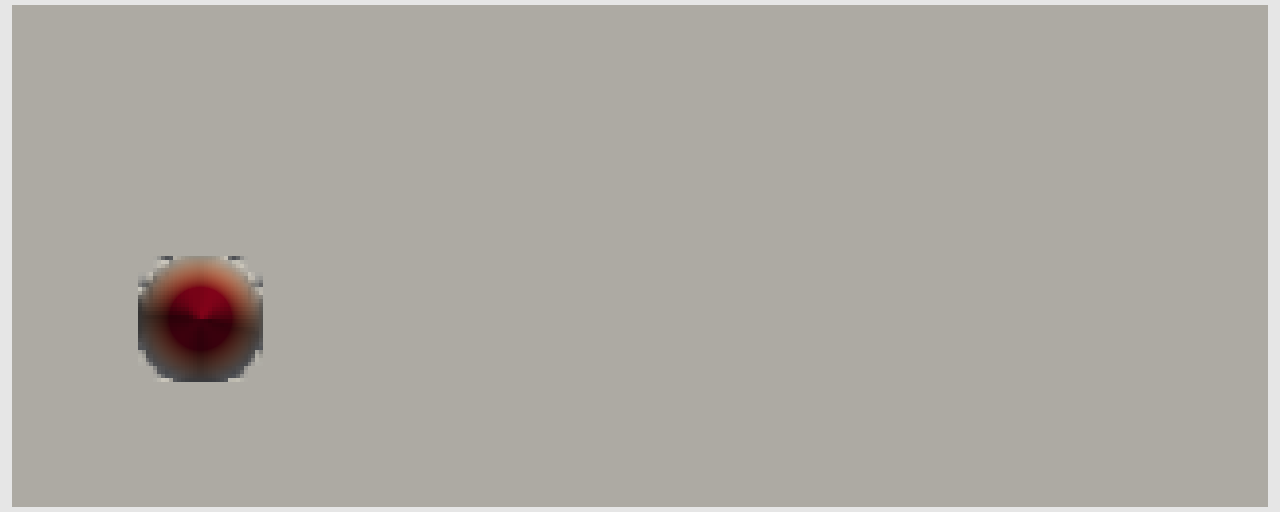
\includegraphics[width=0.499\textwidth]{wave_0}\hfill
%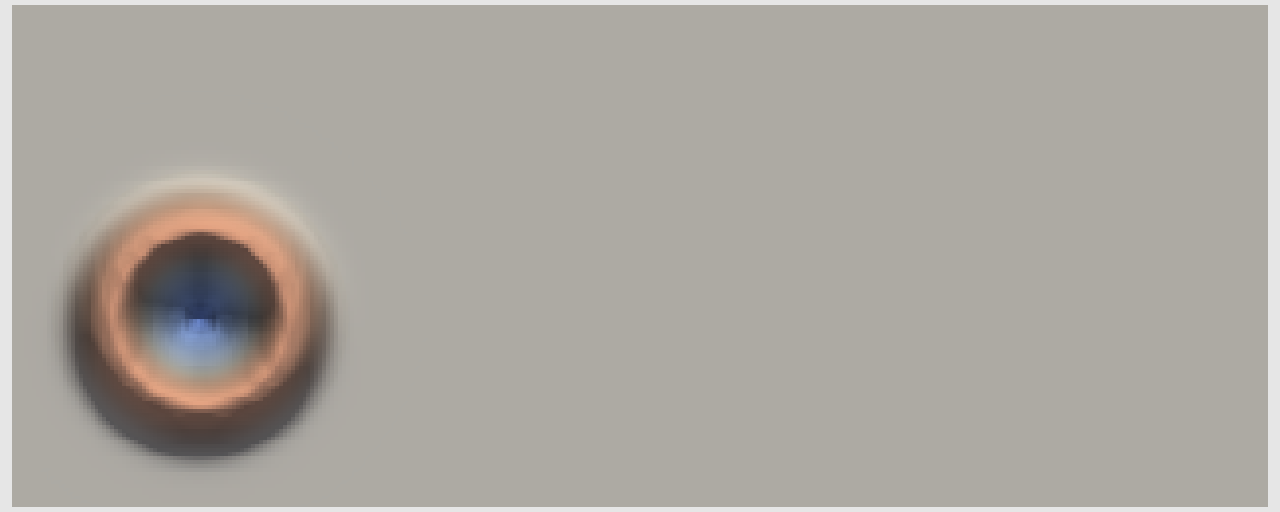
\includegraphics[width=0.499\textwidth]{wave_1}
%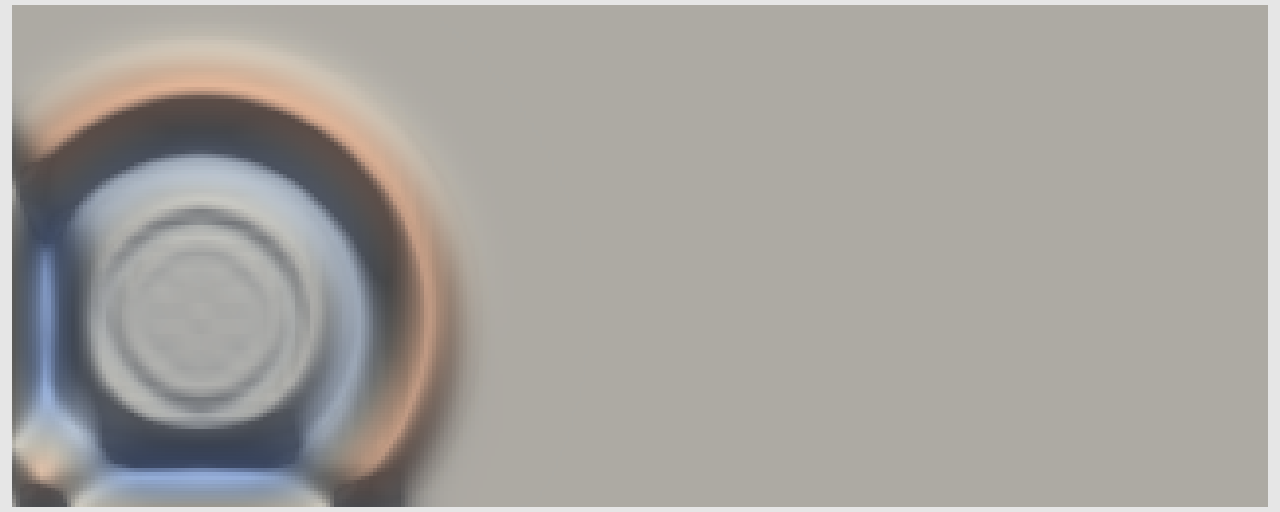
\includegraphics[width=0.499\textwidth]{wave_2}\hfill
%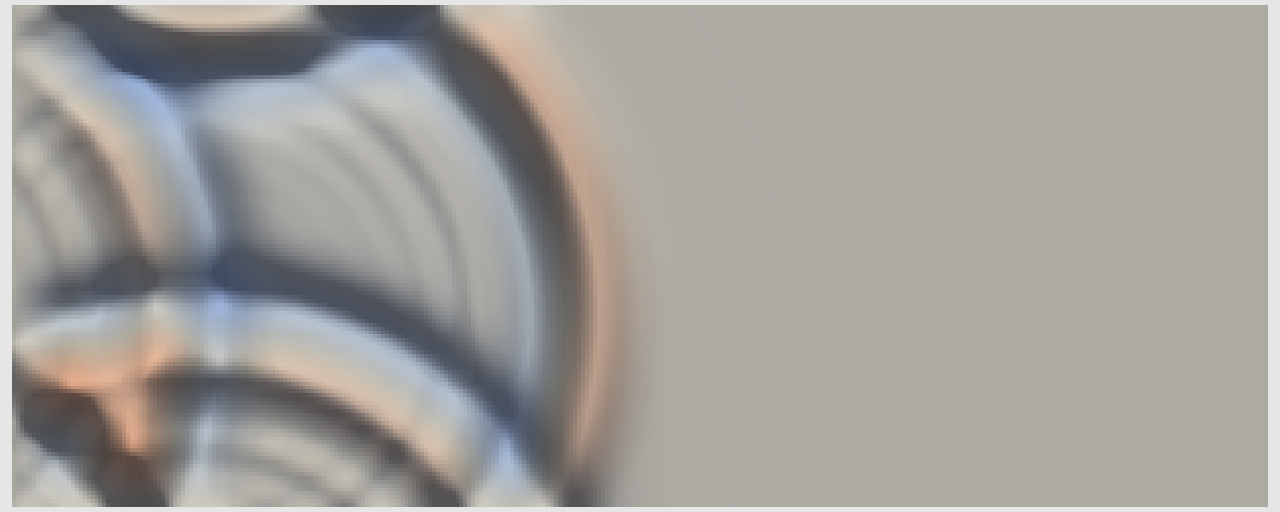
\includegraphics[width=0.499\textwidth]{wave_3}
%\end{center}
%\caption{Solution of the wave equation at four different times. Time is proceeding left
%to right, top to bottom.}
%\label{fig:Bunt}
%\end{figure}

%The example solves the wave equation in the domain
%$\Omega = (0,2.5)\times (0,1)^{d-1}$ with a bump-like
%initial condition. The results for the two-dimensional case are
%illustrated in Figure \ref{fig:Bunt}. The initial bump has a height of 1
%while the color code corresponds to blue for $-0.5$ and red for $0.5$.

\section{Outlook}

The following ideas could be explored from this tutorial:
\begin{itemize}
\item Explore polynomial degree greater than $2$ by changing the blocking
to \lstinline{none}.
\item Compute the total energy $E(t) = \|\partial_t u\|_{0,\Omega}^2 +
  \|\nabla u\|_{0,\Omega}^2$ and check its conservation in
the numerical scheme.
\item Try various time integrators, in particular the Crank-Nicolson method.
\item Implement the elliptic projection method of \cite{Eriksson} from
equation \eqref{eq:Eriksson}.
\end{itemize}

% bibtex bibliography
\bibliographystyle{plain}
\bibliography{tutorial07.bib}

\end{document}
